\chapter{Rappresentazione dei numeri negativi}
\section{Perchè ne abbiamo bisogno?}
Come visto in precedenza, con la modalità di rappresentazione semplice non è possibile rappresentare numeri negativi.

Per ovviare a questo problema sono stati definiti varie modalità di rappresentazione dei numeri interi

\section{MS - Modulo e Segno}
\subsection{Procedura}
Supponiamo di avere a disposizione 1 Byte per rappresentare numeri sia positivi che negativi.

Ricorrendo al metodo del Modulo e Segno utlizzeremo:
\begin{itemize}
    \item I primi 7 bit da destra per il valore assoluto del numero
    \item Il bit più a sinistra (MSB) per indicare il segno
    \begin{itemize}
        \item 1 se il numero è negativo
        \item 0 se è positivo
    \end{itemize}
\end{itemize}

\subsection{Range di rappresentabilità}
Con n bit totali si possono raprpesentare i numeri interi nell'intervallo
{\LARGE
$$
    [-(2^{n-1}-1),\ +(2^{n-1}-1)]_{10}
$$
}

\subsection{Difetti del sistema}
\begin{itemize}
    \item Esistono 2 diverse rappresentazioni dello 0 
    {\Large
        $$
        0000_2 = +0_{10} \qquad 1000_{2} = -0_{10}
    $$}
    \item Un bit tra tutti i bit disponibili viene "speso" per il segno
\end{itemize}

\subsection{Esempio di conversione}
\begin{center}
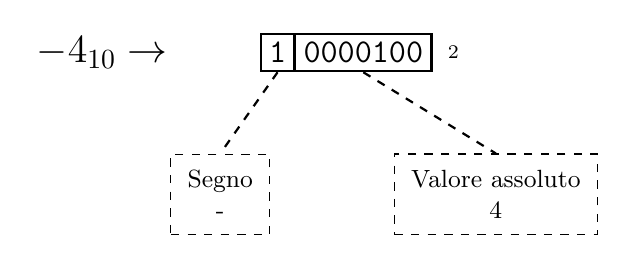
\begin{tikzpicture}[
    box/.style={
        draw,
        thick,
        rectangle,
        inner sep=3pt,
        font=\large\ttfamily
    },
    dashedbox/.style={
        draw,
        dashed,
        rectangle,
        align=center,
        inner sep=6pt,
        font=\small
    }
]

    % Testo a sinistra
    \node (lefttext) at (-2, 0) {\Large $-4_{10} \;\mathbf{\rightarrow}$};

    % Caselle del numero binario
    \node[box, anchor=west] (segno_bit) at (0, 0) {1};
    \node[box, anchor=west, xshift=-0.5pt] (modulo_bit) at (segno_bit.east) {0000100};
    \node[anchor=west, xshift=2pt] at (modulo_bit.east) {$_2$};

    % Box tratteggiati in basso
    \node[dashedbox] (segno_label) at (-0.5, -1.8) {Segno\\-};
    \node[dashedbox] (modulo_label) at (3.0, -1.8) {Valore assoluto\\4};

    % Frecce/linee tratteggiate di collegamento
    \draw[dashed, thick] (segno_bit.south) -- (segno_label.north);
    \draw[dashed, thick] (modulo_bit.south) -- (modulo_label.north);

\end{tikzpicture}
\end{center}

\subsection{Somma}
Come si esegue la somma di 2 valori in Modulo e Segno?

Confronto i bit di segno dei 2 numeri
\begin{enumerate}
    \item Se i bit di segno sono \textbf{uguali}:
    \begin{enumerate}[label=\theenumi.\arabic*.]
        \item Il bit di segno risultante sarà il bit di segno dei due addendi
        \item Eseguo la somma bit a bit dei moduli (a meno di overflow)
    \end{enumerate}
    
    \textbf{Esempio (segni uguali):} $(-2_{10}) + (-3_{10})$ su 4 bit:
    \[
    \begin{array}{r@{\quad}c@{\quad}l}
      \text{Segno} & \text{Modulo} & \\
      \mathbf{1} & 010_2 & (-2_{10}) \\
    + \mathbf{1} & 011_2 & (-3_{10}) \\
    \hline
      \mathbf{1} & 101_2 & (-5_{10})
    \end{array}
    \]

    \item Se i bit di segno sono \textbf{diversi}:
    \begin{enumerate}[label=\theenumi.\arabic*.]
        \item Confronto i valori assoluti
        \item Il bit di segno risultante sarà il bit di segno dell'addendo con valore assoluto maggiore
        \item Eseguo la differenza bit a bit tra il modulo maggiore e quello minore
    \end{enumerate}

    \textbf{Esempio (segni diversi):} $(+3_{10}) + (-2_{10})$ su 4 bit:
    \[
    \begin{array}{r@{\quad}c@{\quad}l}
      \text{Segno} & \text{Modulo} & \\
      \mathbf{0} & 011_2 & (+3_{10}) \\
    + \mathbf{1} & 010_2 & (-2_{10}) \\
    \hline
      \mathbf{0} & 001_2 & (+1_{10})
    \end{array}
    \]
\end{enumerate}

\subsection{Sottrazione}
Come si esegue la sottrazione di due valori in Modulo e Segno:

Confronto i bit di segno dei 2 numeri:
\begin{enumerate}
    \item Se i bit di segno sono \textbf{uguali}:
    \begin{enumerate}[label=\theenumi.\arabic*.]
        \item Il bit di segno risultante sarà uguale al bit di segno dell'operando a modulo maggiore
        \item Il risultato avrà modulo pari alla differenza dei moduli degli operandi (modulo maggiore $-$ modulo minore)
    \end{enumerate}

    \textbf{Esempio (segni uguali):} $(+2_{10}) - (+3_{10})$ su 4 bit:
    \[
    \begin{array}{r@{\quad}c@{\quad}l}
      \text{Segno} & \text{Modulo} & \\
      \mathbf{0} & 010_2 & (+2_{10}, \text{ minuendo}) \\
    - \mathbf{0} & 011_2 & (+3_{10}, \text{ sottraendo}) \\
    \hline
      \mathbf{1} & 001_2 & (-1_{10}, \text{ poich\'e } 3 > 2 \text{ prende il segno del sottraendo})
    \end{array}
    \]

    \item Se i bit di segno sono \textbf{diversi}:
    \begin{enumerate}[label=\theenumi.\arabic*.]
        \item Il bit di segno risultante sarà uguale al bit di segno del minuendo
        \item Il risultato avrà modulo pari alla somma dei moduli dei 2 operandi
    \end{enumerate}

    \textbf{Esempio (segni diversi):} $(+2_{10}) - (-3_{10})$ su 4 bit:
    \[
    \begin{array}{r@{\quad}c@{\quad}l}
      \text{Segno} & \text{Modulo} & \\
      \mathbf{0} & 010_2 & (+2_{10}, \text{ minuendo}) \\
    - \mathbf{1} & 011_2 & (-3_{10}, \text{ sottraendo}) \\
    \hline
      \mathbf{0} & 101_2 & (+5_{10}, \text{ prende il segno del minuendo e somma i moduli})
    \end{array}
    \]
\end{enumerate}




\newpage
\section{CA1 - Complemento a 1}
\subsection{Complemento}
Come indica il nome stesso, questo metodo si basa sull'operazione di \textbf{complemento}.

Con \textbf{complemento} si intende l'operazione che associa ad un un bit il suo opposto, cioè il valore ottenuto sostituendo gli 1 con 0, e tutti gli 0 con 1

\subsection{Procedura}
Il metodo CA1 è motlo semplice e diretto:
\begin{enumerate}
    \item Se il numero da codificare è \textbf{positivo} lo si converte con il metodo binario tradizionale
    \item Se il numero da codificare è \textbf{negativo} basta convertire in binario il suo modulo e quindi eseguire l'operazione di complemento sulla codifica binaria effettuata
\end{enumerate}

\subsection{Range di numeri rappresentabili}
Con n bit totali si possono raprpesentare i numeri interi nell'intervallo
{\LARGE
$$
    [-(2^{n-1}-1),\ +(2^{n-1}-1)]_{10}
$$
}

\subsection{Difetti}
Anche in questo caso sussiste il problema delle due diverse rappresentazioni dell 0
{
    \Large
    \begin{gather*}
    0000\ 0000\, (+0) \\
    1111\ 1111\, (-0)
\end{gather*}}

\subsection{Esempi di conversione}
\begin{itemize}
    \item supponiamo di avere 4 bit e di voler rappresentare in CA1 il valore $3_{10}$
{\large
        \[
        3_{10} = 0011_2
    \]}

    \item supponiamo di avere 4 bit e di voler rappresentare in CA1 il valore $-3_{10}$
   {\large
     \[
        -3_{10} = \overline{0011_2} = 1100_2
    \]}
\end{itemize}

\newpage
\section{CA2 - Complemento a 2}
\subsection{Procedura}
\begin{enumerate}
    \item Se il numero X è \textbf{positivo} esso rimane invariato
    \item Se il numero X è \textbf{negativo}
    \begin{enumerate}[label=\theenumi.\arabic*.]
        \item Si effettua il CA1 sul valore da codificare
        \item Si somma +1 al risultato ottenuto con CA1
    \end{enumerate}
\end{enumerate}

In CA2 i valori negativi hanno MSB = 1

\subsection{Conversione a decimale}
\begin{itemize}
    \item Se il numero è \textbf{positivo} (MSB = 0), si converte in base decimale usando il numero binario puro
    \item Se il numero è \textbf{negativo} (MSB = 1), si applica l'operazione di CA2 a questo valore ottenendo la rappresentazione del corrispondente positivo, si converte il risultato come numero in binario puro e si aggiunge il segno meno
\end{itemize}

\subsection{Range di numeri rappresentabili}
Il metodo CA2 super il principale difetto di CA1, ossia la presenza di una doppia codifica per lo 0.

Dati n bit, si possono rappresentare i numeri interi nell'intervallo
{\LARGE
    $$
    [-(2^{n-1}),\ +(2^{n-1}-1)]
    $$
}
\subsection{Esempi di conversione}
\begin{table}[h!]
\centering
\renewcommand{\arraystretch}{1.3} % Per dare un po' di respiro alle righe
\begin{tabular}{|c|c|c|}
\hline
\textbf{Bit} & \textbf{\begin{tabular}[c]{@{}c@{}}Valore\\ Assoluto\end{tabular}} & \textbf{Complemento a 2} \\ \hline
0111 1111 & 127 & 127 \\ \hline
0111 1110 & 126 & 126 \\ \hline
0000 0010 & 2   & 2   \\ \hline
0000 0001 & 1   & 1   \\ \hline
0000 0000 & 0   & 0   \\ \hline
1111 1111 & 255 & $-1$  \\ \hline
1111 1110 & 254 & $-2$  \\ \hline
1000 0010 & 130 & $-126$ \\ \hline
1000 0001 & 129 & $-127$ \\ \hline
1000 0000 & 128 & $-128$ \\ \hline
\end{tabular}
\end{table}

\subsection{Somma}
Come si esegue la somma di 2 valori in CA2?

\begin{enumerate}
    \item Si esegue la somma su tutti i bit degli addendi, compreso il segno
    \item Un eventuale riporto oltre il bit di segno viene scartato
    \item Nel caso di operandi di segno concorde occorre verificare la presenza o meno di overflow
\end{enumerate}

\subsubsection{Esempio 1}
 $3 + (-8)$
\[
\begin{array}{r@{\quad}c}
  (+3) & 0000\ 0011 \\
+ (-8) & 1111\ 1000 \\
\hline
  (-5) & 1111\ 1011
\end{array}
\]

\subsubsection{Esempio 2}
 $-2 + (-5)$
\[
\begin{array}{r@{\quad}c@{\quad}l}
  (-2) & \phantom{1\ }1111\ 1110 & \\
+ (-5) & \phantom{1\ }1111\ 1011 & \\
\hline
  (-7) & 1\ 1111\ 1001 & \text{: scarto il carry}
\end{array}
\]

\subsection{Sottrazione}
La sottrazione tra 2 numeri in CA2 viene trasformata in somma applicando la regola
{
    \LARGE
    $$
    A - B = A +(-B)
    $$
}
\begin{center}
    \LARGE
    ovvero
\end{center}
{
    \LARGE
    $$
    A - B = A +CA2(B)
    $$
}

Per assicurarsi della correttezza del risultato di un'operazione di somma in CA2 bisogna verificare l'assenza di overflow
\begin{itemize}
    \item Non si ha overflow se gli operandi hanno segno discorde
    \item Si ha overflow se gli operandi hanno segno concorde e il segno del risultato è discorde con essi
\end{itemize}

\newpage
\section{Rappresentazione eccesso $2^{n-1}$}
\subsection{Procedure}
Nella rappresentazione eccesso $2^{n-1}$ un numero X è rappresentato come segue:
$$
    X + 2^{n-1}
$$

\subsubsection{Regola pratica}
I numeri in eccesso $2^{n-1}$ si ottengono da quelli in CA2 complementando il bit più significativo

\subsection{Range numeri rappresentabili}
{\LARGE
    $$
    [-(2^{n-1}),\ +(2^{n-1}-1)]
    $$
}

\subsection{Esempio di conversione}
Vogliamo rappresentare il valore $X = -3$ su $n = 4$ bit.

\subsubsection{Metodo 1: Applicazione della formula $X + 2^{n-1}$}
\begin{enumerate}
    \item Calcoliamo il valore da codificare:
    $$ -3 + 2^{3} = -3 + 8 = 5_{10} $$
    \item Convertiamo il valore $5_{10}$ ottenuto in binario puro a 4 bit:
    $$ 5_{10} = 0101_2 $$
\end{enumerate}

\subsubsection{Metodo 2: Tramite la Regola Pratica (da CA2)}
\begin{enumerate}
    \item Rappresentiamo $X = -3$ in Complemento a 2 (CA2) su 4 bit:
    $$ -3_{10} \xrightarrow{\text{CA2}} \mathbf{1}101_2 $$
    \item Complementiamo (invertiamo) il bit più significativo (MSB):
    $$ \mathbf{1}101_2 \xrightarrow{\text{inverti MSB}} \mathbf{0}101_2 $$
\end{enumerate}

\newpage
\section{Rappresentazione Eccesso 128}
\subsection{Procedura}
Nella rappresentazione Eccesso 128 un numero X è rappresentato come segue:
$$
    X + 128
$$

\subsection{Esempi}

\[
\begin{array}{r@{\qquad}c@{\qquad}l}
    X = 5 & 5 + 128 = 133 & 1000\ 0101_2 \\[0.5em]
    X = -3 & -3 + 128 = 125 & 0111\ 1101_2
\end{array}
\]

\paragraph{Passando da CA2:}
\[
-3_{10} 
\longrightarrow \overbrace{00000011_2}^{3} 
\longrightarrow \overbrace{11111100_{\text{CA2}}}^{\bar{*3}} 
\xrightarrow{\quad\text{CA2}\quad} \overbrace{11111101_{\text{CA2}}}^{-3} 
\xrightarrow{\substack{\text{complemento il bit}\\\text{più significativo}}} \overbrace{\mathbf{0}1111101_{\text{Eccesso}128}}^{-3}
\]

\subsection{Osservazioni}

\begin{itemize}
    \item In Eccesso 128 i numeri da $[-128, 127]$ si mappano su $[0, 255]$
    \item In Eccesso, usa una convenzione per il bit di segno opposta: 0 per i numeri negativi e 1 per quelli positivi.
\end{itemize}